\documentclass[10pt, compress]{beamer}

\usetheme{m}

\usepackage[utf8]{inputenc}
\usepackage[french]{babel}
\usepackage[T1]{fontenc}
\usepackage{booktabs}
\usepackage[scale=2]{ccicons}
\usepackage{minted}
\usepackage{tikz}
\usepackage[ruled,vlined,english]{algorithm2e}
\usetikzlibrary{arrows,automata,shapes,positioning,calc}

\usepackage{float} % placement des figures
\usepackage{amssymb} % symboles mathématiques
\usepackage{textcomp} % flèche,  intervalle
\usepackage{stmaryrd} % intervalle entiers
\usepackage{graphicx} % affichage d'images
\usepackage{url} % inclure des urls
\usepackage{forest}

\newcommand{\first}{\texttt{First}}
\newcommand{\last}{\texttt{Last}}
\newcommand{\sort}{\texttt{Sort}}
\newcommand{\triple}{\texttt{Triple}}
\newcommand{\produ}{\texttt{Normalize}}

\newenvironment{exemple}
{\begin{exampleblock}{Example}}
{\end{exampleblock}}

\newenvironment{defi}
{\begin{block}{Definition}}
{\end{block}}

\usepgfplotslibrary{dateplot}

\usemintedstyle{trac}

\title{Platypus}
\subtitle{L'outil libre qui répond à vos questions}
\date{JDLL 2015}    

\begin{document}

\maketitle

The {\em Projet Pensées Profondes} (Deep Thought Project) aims at
providing a powerful software for answering questions written in
natural language.
To accomplish this, we developped an eponymous set of tools that
accomplish different tasks and fit together thanks to a protocol
we developped.

These various tasks include data querying (using the young and open
knownledge base Wikidata), question parsing (using the
CoreNLP software written by Stanford University and machine learning),
requests routing, web user interface, and feedback reporting.

Given the young age of this projet, these pieces are only starting
to emerge with their first features and mutual communications,
so we will describe them separately in this document without
much of a general overview of the project.


\section{Aperçu}
\begin{frame}[fragile]
    \frametitle{Architecture}
    \begin{figure}
        \resizebox{.9\linewidth}{!}{
            \newlength{\moduledistance}
\setlength{\moduledistance}{1cm}
\overfullrule=2cm
\tikzset{
    module/.style={
           rectangle,
%           rounded corners,
           draw=mDarkTeal, very thick,
           minimum width=3cm,
           minimum height = 0.7cm,
           node distance = 1.5cm,
           inner sep=2pt,
           text centered,
           },
}

\tikzset{
    core/.style={
           circle,
           draw=mDarkTeal, very thick,
           minimum width=2cm,
           inner sep=2pt,
           text centered,
           },
}

\tikzset{
    arrow/.style={
           ->,
           draw=mDarkTeal, very thick,
    }
}

\tikzset{
    darrow/.style={
           <->,
           draw=mDarkTeal, very thick,
    }
}

\begin{tikzpicture}[->,>=stealth']
    \node[core] (core) {
        Core
    };
    \node[module,
          right of=core,
          right=\moduledistance,
          ] (grammatical) {
          Grammatical
    };
    \node[module,
          below of=grammatical,
          ] (standalone) {
        \begin{tabular}{c}
        Machine Learning\\Standalone
        \end{tabular}
    };
    \node[module,
          above of=grammatical,
          ] (reformulation) {
        \begin{tabular}{c}
        Machine Learning\\Reformulation
        \end{tabular}
    };
    \node[module,
          left of=core,
          left=\moduledistance,
          ] (wikidata) {
        Wikidata
    };
    \node[module,
          above of=wikidata,
          ] (cas) {
        Computer Algebra
    };
    \node[module,
          below of=wikidata,
          ] (spellchecker) {
        Spell-checker
    };
    \node[module,
          above of=core,
          above=1cm,
          ] (webui) {
        \begin{tabular}{c}
        Web User\\
        Interface
        \end{tabular}
    };
    \node[module,
          above of=reformulation,
%          right=\moduledistance,
          ] (logging) {
        Logging backend
    };
    \draw[mLightBrown,thick] ($(reformulation.north west)+(-0.3,0.3)$)  rectangle node[yshift=-2.5cm,below] {Question Parsing} ($(standalone.south east)+(0.3,-0.3)$);
    \draw[mLightBrown,thick] ($(cas.north west)+(-0.3,0.3)$)  rectangle node[yshift=-2.5cm,below] {Other modules} ($(spellchecker.south east)+(0.3,-0.3)$);

    \draw [darrow] (core)          -- node{} (cas.south east);
    \draw [darrow] (core)          -- node{} (wikidata.east);
    \draw [darrow] (core)          -- node{} (spellchecker.north east);
    \draw [darrow] (core)          -- node{} (reformulation.south west);
    \draw [darrow] (core)          -- node{} (grammatical.west);
    \draw [darrow] (core)          -- node{} (standalone.north west);
    \draw [darrow] (core)          -- node{} (webui.south);
    \draw [darrow] (webui)         -- node{} (logging.west);
    \draw [arrow]  (logging)       -- node{} (reformulation.north);
    \draw [arrow]  (grammatical)   -- node{} (reformulation.south);

\end{tikzpicture}

        }
    \end{figure}
\end{frame}

\begin{frame}[fragile]
    \frametitle{Datamodel}
    How to represent formally a question asked in natural language?

    \alert{Tree} structure.
\end{frame}
\begin{frame}[fragile]
    \frametitle{Datamodel \--- Leaves: resources}
        \begin{itemize}
            \item Strings: "Isaac \textsc{Newton}"
            \item Dates: 25 December 1642
            \item Geographic coordinates: 47° 30' 18'' N ; 9° 44' 57'' E
            \item \ldots
        \end{itemize}
\end{frame}
\begin{frame}[fragile]
    \frametitle{Datamodel \--- Nodes: operations}
        \begin{itemize}
            \item Full \alert{triples}: (Isaac \textsc{Newton}, birth date, 25 December 1642 (Julian)) $\rightarrow$ true
            \item Missing: (?, birth date, 25 December 1642 (Julian)) $\rightarrow$ [Isaac \textsc{Newton}]
            \item Union, Intersection, Difference, \ldots
            \item And, Or, Not
            \item Exists
            \item Sort, First, Last
        \end{itemize}
\end{frame}

\begin{frame}[fragile]
    \frametitle{Datamodel \--- Examples}
    \begin{itemize}
        \only<1>{
        \item \alert{"Is Brussels the capital of Belgium and the European Union?"}
          \begin{center}
            \begin{figure}
          \resizebox{\linewidth}{!}{
            \begin{tikzpicture}
              \node (0) at (10,8.5) {$\bigwedge$};
              \node (1) at (7,7) {$\triple$};
              \node (11) at (5,5.5) {Brussels};
              \node (12) at (7,5.5) {capital};
              \node (13) at (9,5.5) {Belgium};
              
              \node (2) at (13,7) {$\triple$};
              \node (21) at (11,5.5) {Brussels};
              \node (22) at (13,5.5) {capital};
              \node (23) at (15,5.5) {European Union};

              \node (9) at (14,1) {}; % utilisé pour forcer le positionnement de la figure globale

              \draw[->, >=latex] (0) edge node[sloped, anchor=center, above] {} (1);
              \draw[->, >=latex] (1) edge node[sloped, anchor=center, above] {\scriptsize{subj.}} (11);
              \draw[->, >=latex] (1) edge node[sloped, anchor=center, above] {\scriptsize{pred.}} (12);
              \draw[->, >=latex] (1) edge node[sloped, anchor=center, above] {\scriptsize{obj.}} (13);
              \draw[->, >=latex] (0) edge node[sloped, anchor=center, above] {} (2);
              \draw[->, >=latex] (2) edge node[sloped, anchor=center, above] {\scriptsize{subj.}} (21);
              \draw[->, >=latex] (2) edge node[sloped, anchor=center, above] {\scriptsize{pred.}} (22);
              \draw[->, >=latex] (2) edge node[sloped, anchor=center, above] {\scriptsize{obj.}} (23);
             \end{tikzpicture}
            }
            \end{figure}

          \end{center}}
            
        \only<2>{
        \item \alert{"Who is the mayor of the capital of Kreis Bergstraße?"}
          \begin{center}
            \begin{forest}
              [\texttt{Triple}[\texttt{Triple}[Kreis Bergstraße][capital][?]][mayor][?]]
            \end{forest}
          \end{center}}
            
        \only<3>{
          \item \alert{"What is the birth date of the first president of Germany?"}
          \begin{center}
            \begin{forest}
              [\texttt{Triple}[\texttt{First}[\texttt{Sort}[\texttt{Triple}[Germany][president][?]][mandate begin date]]][birth date][?]]
            \end{forest}
          \end{center}}

        \only<4>{
          \item \alert{"Is there a medical treatment for Ebola?"}
            \begin{center}
              \begin{forest}
                [\texttt{Exists}[\texttt{Triple}[Ebola][medical treatment][?]]]
              \end{forest}
            \end{center}}

        \only<5>{
          \item \alert{"Who are the children of François \textsc{Mitterrand} and Anne \textsc{Pingeot}?"}
            \begin{center}
              \begin{forest}
                [$\bigcap$[\texttt{Triple}[François \textsc{Mitterrand}][child][?]][\texttt{Triple}[Anne \textsc{Pingeot}][child][?]]]
              \end{forest}
            \end{center}}


    \end{itemize}
\end{frame}



\begin{frame}[fragile]
    \frametitle{Nested question}

Who is the wife of the president of the United States?
    \begin{tabular}{ll}
        \alert{WolframAlpha} & Barack Obama\\
        \alert{Platypus} & Michelle Obama\\
    \end{tabular}

    \medbreak

    What are the birth dates of the daughters of the wife of the president of the United States?
    \begin{tabular}{ll}
        \alert{WolframAlpha} & Barack Obama\\
        \alert{Platypus} & Saturday, July 4, 1998 \& Sunday, June 10, 2001\\
    \end{tabular}
\end{frame}

\begin{frame}[fragile]
    \frametitle{Conjunction}

Who is an actor in Titanic and Inception?
    \begin{tabular}{ll}
        \alert{WolframAlpha} & all the actors of the two movies\\
        \alert{Platypus} & Leonardo DiCaprio\\
    \end{tabular}
\end{frame}

\section{Future work}

\begin{frame}[fragile]
    \frametitle{Better database}

    ``How fast is the TGV?''

    ``How wide is a tennis court?''

    Not answered by \alert{Wikidata}.

    \medbreak

    $\rightarrow$ Improve Wikidata?

    $\rightarrow$ Use another database?
\end{frame}

\begin{frame}[fragile]
    \frametitle{Better question parsing}

    ``What is the date of birth of Isaac Newton?''

    ``In which band does Bono sing?''

    Not parsed correctly.

    \medbreak

    $\rightarrow$ Train the Stanford CoreNLP library?

    $\rightarrow$ Improve the algorithm of the Grammatical module?

    $\rightarrow$ Better datasets for the ML modules?
\end{frame}

\begin{frame}[fragile]
    \frametitle{New modules}
    \begin{table}
    \Large
    \centering
    \begin{tabular}{ccc}
        \textcolor{mLightBrown}{cooking recipes} & \textcolor{mDarkBrown}{HAL} & \textcolor{mMediumBrown}{meteo} \\
        \multicolumn{3}{c}{\textcolor{mDarkTeal}{programming language interpreter}} \\
        \textcolor{mMediumBrown}{cinema} & \textcolor{mDarkTeal}{music} & \textcolor{mLightBrown}{literature}\\
        \textcolor{mDarkBrown}{OEIS} & \textcolor{mLightBrown}{translation} & \textcolor{mDarkTeal}{chemistry}\\
        \multicolumn{3}{c}{\textcolor{mMediumBrown}{sport statistics and predictions}} \\
    \end{tabular}
    \end{table}
\end{frame}

\begin{frame}[fragile]
    \frametitle{Some facts} % to update just before the presentation
    \alert{23 repositories}

    \begin{tabular}{lll}
        6 & PHP & Wikidata libraries and module\\
        12 & Python & Other modules, core, and libraries\\
        1 & C++ & ML-Reformulation\\
        1 & Shell & Deployment scripts\\
        1 & \LaTeX & This presentation and the report\\
        1 & Markdown & The specification\\
        1 & HTML/CSS/Javascript & The Web User Interface\\
        1 & HTML/CSS & The project's website\\
    \end{tabular}

    \alert{1982 commits} (without the ``integration'' repository, which has an automatic commit every 12h)

    \alert{26k lines} of code (13k in PHP, 10k in Python)
\end{frame}

\newlength{\logosize}
\setlength{\logosize}{12pt}
\begin{frame}[fragile]
    \frametitle{Stay tuned}
    \alert{\url{http://projetpp.github.io/}}

    \begin{tabular}{ll}
        
\includegraphics[width=\logosize]{Twitter_logo_blue.png} & \href{https://twitter.com/ProjetPP}{https://twitter.com/ProjetPP}\\
        
\includegraphics[width=\logosize]{GitHub-Mark-32px.png} &  \href{https://github.com/ProjetPP}{https://github.com/ProjetPP}\\
        
\includegraphics[width=\logosize]{ic_email_black_18dp.png} & \href{mailto:ppp@pony.ovh}{ppp@pony.ovh}\\
    \end{tabular}
\end{frame}


\begin{frame}
    \frametitle{Questions?}
    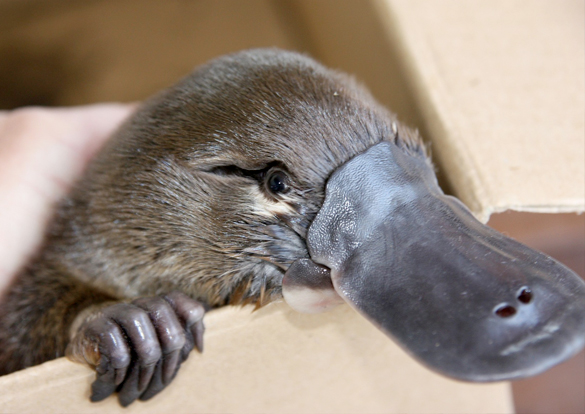
\includegraphics[width=\linewidth]{figures/platypusLg.jpg}
\end{frame}


\end{document}
